\documentclass[11pt,a4paper]{article}
\usepackage[margin=1in]{geometry}
\usepackage[T2A]{fontenc}
\usepackage[utf8]{inputenc}
\usepackage[english,russian]{babel}
\usepackage{amsmath,amssymb}
\usepackage{graphicx}
\usepackage{microtype}
\usepackage{hyperref}

\hypersetup{
  pdftitle={Численная оптимизация двухкомпонентного профиля Field 01 на фиксированном фоне},
  pdfauthor={Nikolai Dereviankin},
  pdfcreator={LaTeX},
  pdfproducer={pdfTeX}
}

\setlength{\parindent}{0pt}
\setlength{\parskip}{0.75\baselineskip}
\renewcommand{\arraystretch}{1.2}
\graphicspath{{figures/}{../figures/}}
\sloppy

\title{Численная оптимизация двухкомпонентного профиля Field 01 на фиксированном фоне\\
\large Checkpoint v0.4: локализаторы, ворота допуска, замыкание координат и воспроизводимость}
\author{Николай Деревянкин}
\date{}

\newcommand{\xibr}{\xi_{\mathrm{br,max}}}
\newcommand{\vac}{V}
\newcommand{\host}{H}
\newcommand{\ldiff}{L_{\Delta}}
\newcommand{\lalign}{L_{\mathrm{A}}}

\begin{document}
\maketitle

\begin{center}
\textit{Рабочий численный отчёт v0.4 --- редакция 2026-08-07}
\end{center}

\begin{abstract}
В работе фиксируется завершённый этап ограниченной численной оптимизации двухкомпонентного локализатора Field 01 на фиксированном фоне. Рассматриваются два независимых канала деформации: знакопеременный difference-локализатор, управляющий относительным профилем двух компонентов, и aligned-локализатор, управляющий их согласованной деформацией. Для обоих каналов выписаны фактически использованные семейства функций, включая линейные, квадратичные и кубически-экспоненциальные направления. Кандидаты принимались только после структурного и спектрально-физического контроля, проверки прогнозируемого прироста, сопоставления радиусов и прямой проверки точки поворота ветви (fold). Сохранённый результат равен $\xibr=2.0934591793773114\times10^{-3}$ и улучшает контрольную точку (checkpoint) v0.3 на $1.218886\%$. Девять выбранных координат замкнуты по заранее установленному порогу прямой проверки $1\%$. Отчёт не утверждает глобальную оптимальность, не вводит фундаментальное действие и не заменяет полный анализ статической обратной реакции или динамической устойчивости.
\end{abstract}

\textbf{Ключевые слова:} Field 01; двухкомпонентный локализатор; фиксированный фон; численная оптимизация; продолжение ветви; точка поворота; прогнозирующая модель; сопоставление радиусов; замыкание координат; воспроизводимость.

\section{Статус и цель отчёта}

Этот текст документирует конкретную численную контрольную точку (checkpoint), а не завершённую физическую теорию. Его цель состоит в том, чтобы отделить реально вычисленный результат от более широкого интерпретационного языка Field 01 и представить процедуру оптимизации в форме, пригодной для независимой проверки.

Объектом оптимизации является ограниченное семейство локализаторов в ранее выбранной двухкомпонентной задаче на фиксированном фоне (fixed-background). Фоновые уравнения, граничные условия и сектор решения сохраняются неизменными. Меняется только форма двух локализующих направлений внутри заранее определённого параметрического семейства (ansatz).

Величина $\xibr$ является внутренней безразмерной диагностикой максимума связанной ветви обратной реакции. Она не является экспериментально измеренной наблюдаемой величиной и в текущем отчёте не отождествляется с массой, зарядом, вероятностью существования частицы или иной физической наблюдаемой.

\section{Ограниченное пространство профилей}

Пусть $\host\in[0,1]$ обозначает нормированную переменную базового профиля (host), а
\begin{equation}
\vac(\host)=1-\host^2
\end{equation}
--- соответствующее расстояние до вакуумного края в пространстве профиля. В используемом параметрическом семействе деформации разделены на разностный (difference) и согласованный (aligned) каналы.

\subsection{Difference-локализатор}

Знакопеременный локализатор записывается как
\begin{equation}
\ldiff(\host)
=\vac^q
+d\,B_{\Delta}(\host),
\label{eq:difference_localizer}
\end{equation}
где
\begin{equation}
B_{\Delta}(\host)
=A_{\Delta}\host^2\vac^s
\left(1-\zeta\host^2\right)
\left(1+c_{1,\Delta}\vac+c_{2,\Delta}\vac^2\right)
\exp\!\left(\lambda\vac^3\right).
\label{eq:difference_basis}
\end{equation}

Нормировка выбирается по условию
\begin{equation}
A_{\Delta}^{-1}
=\max_{\host\in[0,1]}
\left|
\host^2\vac^s
\left(1-\zeta\host^2\right)
\left(1+c_{1,\Delta}\vac+c_{2,\Delta}\vac^2\right)
\exp\!\left(\lambda\vac^3\right)
\right|.
\end{equation}

Параметр $q$ задаёт жёсткость центральной части профиля (core), $d$ --- вес знакопеременного плеча, $\zeta$ --- положение внутреннего узла, $s$ --- степень затухания плеча у вакуумного края, $c_{1,\Delta}$ и $c_{2,\Delta}$ --- линейную и квадратичную ширину, а $\lambda$ --- неполиномиальный кубически-экспоненциальный наклон.

\subsection{Aligned-локализатор}

Согласованный канал имеет вид
\begin{equation}
\lalign(\host)
=A_{\mathrm{A}}\host^2\vac^p
\left(1+c_{1,\mathrm{A}}\vac+c_{2,\mathrm{A}}\vac^2\right)
\exp\!\left(\rho\vac^3\right),
\label{eq:aligned_localizer}
\end{equation}
где
\begin{equation}
A_{\mathrm{A}}^{-1}
=\max_{\host\in[0,1]}
\left[
\host^2\vac^p
\left(1+c_{1,\mathrm{A}}\vac+c_{2,\mathrm{A}}\vac^2\right)
\exp\!\left(\rho\vac^3\right)
\right].
\end{equation}

Здесь $p$ задаёт степень оболочки (shell), $c_{1,\mathrm{A}}$ и $c_{2,\mathrm{A}}$ --- полиномиальные направления ширины, а $\rho$ --- независимый кубически-экспоненциальный наклон согласованного профиля.

Функции \eqref{eq:difference_localizer} и \eqref{eq:aligned_localizer} являются параметрическими локализаторами внутри выбранной численной задачи. Они не объявляются фундаментальными полями и сами по себе не задают действие модели.

Профили такого типа имеют известные аналоги в вихревых и нетопологических солитонных задачах, однако существование и устойчивость локализованного решения зависят от конкретного действия и не следуют из одной формы ansatz \cite{derrick1964,nielsen1973,coleman1985}.

\section{Протокол оптимизации}

Оптимизация проводилась последовательно по одной параметрической координате. Новый кандидат не принимался только потому, что его прогноз (predictor) превышал текущий рекорд. Для перехода к прямому вычислению точки поворота требовалось пройти несколько независимых ворот допуска. Общий численный контекст продолжения ветвей и решения нелинейных краевых задач описан, например, в работах \cite{keller1977,ascher1995}; настоящий отчёт фиксирует собственную ограниченную реализацию этих идей.

\subsection{Структурный контроль}

Проверялись вещественность, гладкость, конечность нормировки, восстановление контрольного профиля при нулевом значении новой координаты и независимость нового касательного направления от уже закрытых полиномиальных направлений. Неполиномиальные множители $\exp(\lambda\vac^3)$ и $\exp(\rho\vac^3)$ положительны для всех вещественных значений параметра, однако положительность множителя не заменяет физическую проверку полного кандидата.

\subsection{Fixed-background физический контроль}

На фиксированном фоне кандидат должен сохранять выбранный спектральный сектор: одну допустимую отрицательную моду, положительную следующую моду, достаточные доли компонент, когерентность, aligned-долю и локализацию. Значения, отделённые от контрольной точки областью нарушения этих условий, не считаются частью той же физически связанной ветви.

\subsection{Кубический predictor}

Для широкого предварительного скрининга использовалась амплитудная координата
\begin{equation}
x=f_{\mathrm{center}}-1
\end{equation}
и локальная модель отклика без свободного постоянного члена:
\begin{equation}
\xi_{\mathrm{br}}(x)
=\chi_1x+\chi_2x^2+\chi_3x^3.
\label{eq:cubic_predictor}
\end{equation}

Коэффициенты определялись по четырём точкам $x=0,0.01,0.02,0.03$, расположенным до измеренного поворота ветви. Первое положительное стационарное значение с отрицательной второй производной использовалось как прогноз точки поворота. Максимальная калибровочная ошибка такого правила скрининга составляла менее $1\%$ на контрольных ветвях.

Прямой fold разрешался только тогда, когда прогнозируемый прирост относительно подтверждённого рекорда достигал заранее установленного порога
\begin{equation}
g_{\mathrm{pred}}
=\frac{\xi_{\mathrm{pred}}}{\xi_{\mathrm{record}}}-1
\geq 0.01.
\label{eq:one_percent_gate}
\end{equation}

\subsection{Прямой fold и matching radii}

Финальный кандидат проверялся прямой процедурой продолжения ветви (continuation). Максимум считался точкой поворота (fold) только при наличии соседних точек с меньшим значением $\xi_{\mathrm{br}}$. Контроль повторялся на радиусах
\begin{equation}
R\in\{30,40,50\}.
\end{equation}

Дополнительно требовались прохождение контроля невязки (residual), закона Гаусса, производной источника, гессиана и знакопеременности, обнаружение точки поворота на каждом радиусе и малая относительная дисперсия результата между радиусами.

\section{Сохранённый checkpoint v0.4}

Итоговый профиль имеет параметры
\begin{center}
\begin{tabular}{@{}lll@{}}
\textbf{Канал} & \textbf{Параметр} & \textbf{Сохранённое значение} \\
\hline
difference & $q$ & $16$ \\
difference & $d$ & $4$ \\
difference & $s$ & $1$ \\
difference & $\zeta$ & $1.8105828289285173$ \\
difference & $c_{1,\Delta}$ & $1.20$ \\
difference & $c_{2,\Delta}$ & $0$ \\
difference & $\lambda$ & $-0.35$ \\
aligned & $p$ & $1$ \\
aligned & $c_{1,\mathrm{A}}$ & $-3.260$ \\
aligned & $c_{2,\mathrm{A}}$ & $3.041$ \\
aligned & $\rho$ & $0$ \\
\end{tabular}
\end{center}

На рисунке~\ref{fig:retained_localizers} показана форма обоих сохранённых локализаторов в одной и той же нормированной координате $\host$.

\begin{figure}[htbp]
\centering
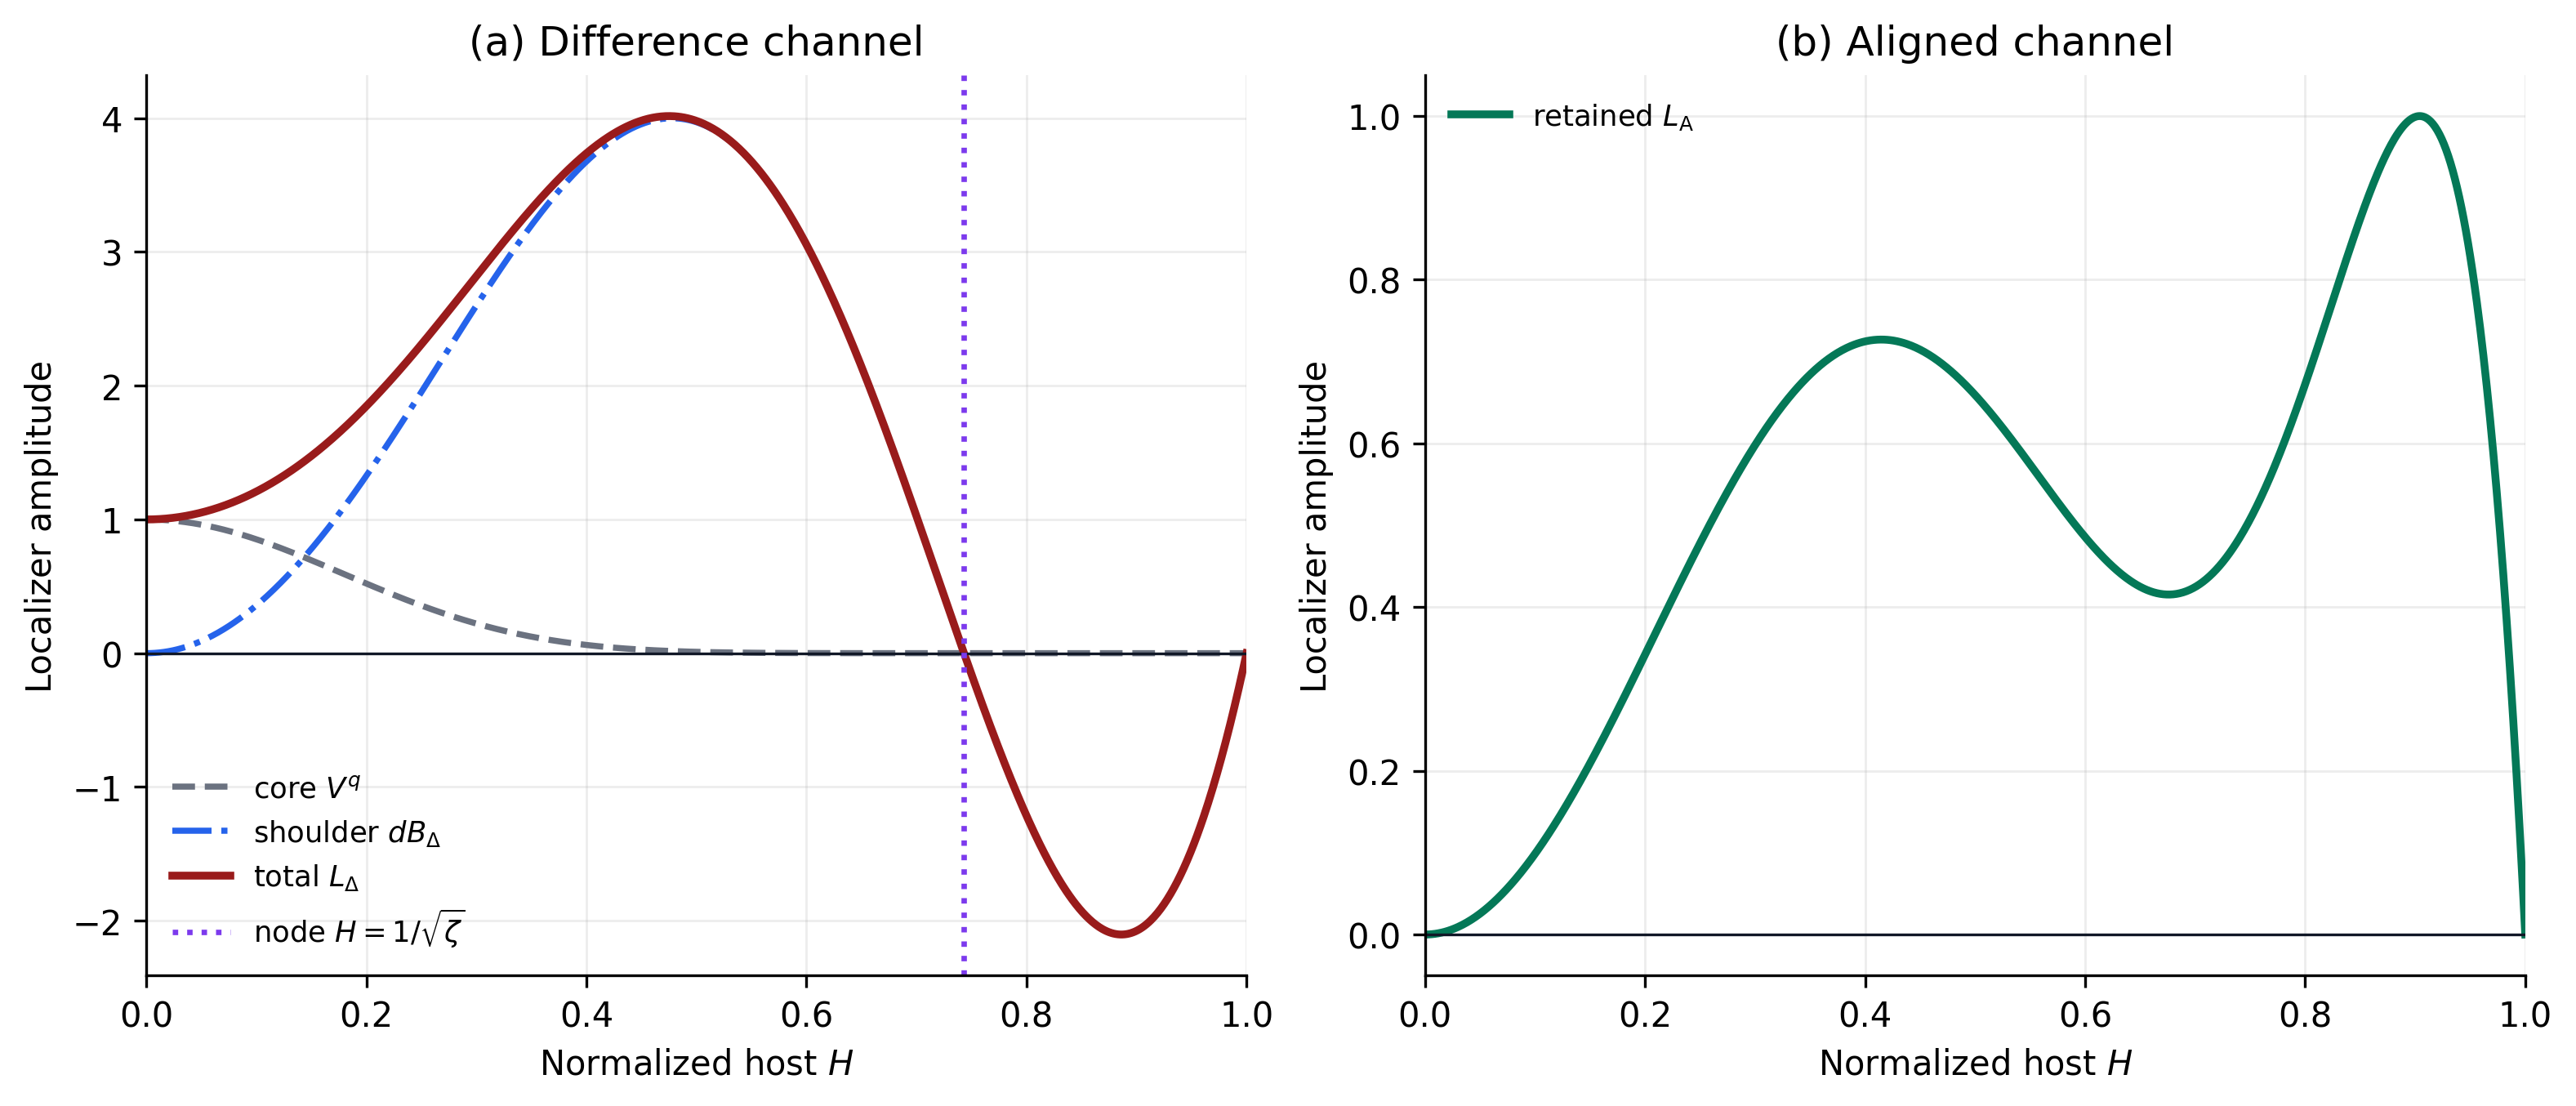
\includegraphics[width=\textwidth]{fixed_background_v0_4_retained_localizers.png}
\caption{Сохранённые локализаторы checkpoint v0.4. (a) Разностный канал: центральный вклад $\vac^q$, знакопеременное плечо $dB_{\Delta}$ и их сумма $\ldiff$; пунктирная вертикаль отмечает внутренний узел $\host=1/\sqrt{\zeta}$. (b) Нормированный согласованный локализатор $\lalign$. Кривые представляют функции выбранного параметрического семейства, а не самостоятельные фундаментальные поля.}
\label{fig:retained_localizers}
\end{figure}

Прямо измеренный максимум равен
\begin{equation}
\boxed{\xibr=2.0934591793773114\times10^{-3}}.
\label{eq:retained_fold}
\end{equation}

Предыдущий checkpoint v0.3 имел
\begin{equation}
\xibr^{(0.3)}=2.0682495692869894\times10^{-3}.
\end{equation}
Относительное улучшение составляет
\begin{equation}
\frac{\xibr}{\xibr^{(0.3)}}-1
=1.218886\%.
\end{equation}

Новый рекорд был получен после введения разностного множителя $\exp(\lambda\vac^3)$ и прямой проверки точки $\lambda=-0.35$.

\section{Эволюция численного рекорда}

В таблице приведены выбранные сохранённые этапы. Она не является полным журналом всех внутренних срезов.

\begin{center}
\small
\begin{tabular}{@{}p{0.34\textwidth}p{0.20\textwidth}p{0.38\textwidth}@{}}
\textbf{Этап} & \textbf{$\xibr$} & \textbf{Роль внутри параметрического семейства} \\
\hline
Однокомпонентный базис ядра & $\approx7.624\times10^{-4}$ & Базовый предел предшествующего однокомпонентного сектора \\
Связанная двухкомпонентная граница & $1.278178674\times10^{-3}$ & Введение компенсирующего плеча \\
Замыкание узла и разностной ширины & $1.307068707\times10^{-3}$ & Разделение областей ядра и плеча \\
Линейная ширина aligned-канала & $1.996071538\times10^{-3}$ & Тонкая настройка согласованного профиля \\
Пересечение benchmark $2\times10^{-3}$ & $2.002226282\times10^{-3}$ & Первая сохранённая точка поворота выше внутреннего benchmark \\
Полиномиальное замыкание aligned-канала v0.3 & $2.068249569287\times10^{-3}$ & Итоговый полиномиальный профиль \\
Кубически-экспоненциальный difference-канал v0.4 & $2.093459179377\times10^{-3}$ & Прямо подтверждённое неполиномиальное улучшение \\
\end{tabular}
\end{center}

\section{Прямая валидация рекорда}

Для сохранённой точки поворота получены следующие диагностические величины:
\begin{align}
\text{predictor relative error} &= 0.057938\%, \\
\text{maximum matching-radius spread} &= 0.074515\%.
\end{align}

На всех трёх радиусах обнаружены точки поворота. Проверка прогноза, ворота сопоставления радиусов и ворота знакопеременной точки поворота пройдены. Эти тесты подтверждают внутреннюю воспроизводимость результата внутри выбранной fixed-background задачи, но не заменяют решение полностью самосогласованной статической системы с обратной реакцией.

\section{Замыкание девяти координат}

Координата называется замкнутой, если после локального скрининга и обязательных физических ворот она не даёт прироста, достаточного для авторизации нового прямого вычисления точки поворота. Максимальный остаточный прирост каждой координаты приведён относительно подтверждённого рекорда.

\begin{center}
\small
\begin{tabular}{@{}p{0.48\textwidth}p{0.18\textwidth}p{0.18\textwidth}@{}}
\textbf{Координата} & \textbf{Значение} & \textbf{Остаточный gain} \\
\hline
Difference cubic-exponential tilt $\lambda$ & $-0.35$ & $0.061392\%$ \\
Difference core power $q$ & $16$ & $0.022068\%$ \\
Difference shoulder coefficient $d$ & $4$ & $0.064457\%$ \\
Difference linear width $c_{1,\Delta}$ & $1.20$ & $0.032797\%$ \\
Difference quadratic width $c_{2,\Delta}$ & $0$ & $0.002023\%$ \\
Aligned shell power $p$ & $1$ & $0$ \\
Aligned linear width $c_{1,\mathrm{A}}$ & $-3.260$ & $0.000274\%$ \\
Aligned quadratic width $c_{2,\mathrm{A}}$ & $3.041$ & $0.012141\%$ \\
Aligned cubic-exponential tilt $\rho$ & $0$ & $0.917518\%$ \\
\end{tabular}
\end{center}

Все значения остаются ниже порога \eqref{eq:one_percent_gate}. Следовательно, в текущем пространстве профилей новое прямое вычисление точки поворота не авторизовано.

\section{Пограничный aligned-сектор}

Наиболее близким к порогу остаётся aligned-множитель
\begin{equation}
\exp\!\left(\rho\left(1-\host^2\right)^3\right).
\end{equation}

Связанная физическая ветвь проходит при $\rho=0.29$ и нарушает физические ворота при $\rho=0.30$. Квадратичная аппроксимация точек $\rho=0.26,0.27,0.28$ даёт
\begin{align}
\rho_{\mathrm{vertex}} &= 0.269251036968, \\
\xi_{\mathrm{pred}} &= 2.112667042958\times10^{-3}, \\
g_{\mathrm{raw}} &= 0.917518\%, \\
g_{\mathrm{calibrated}} &= 0.859580\%.
\end{align}

Необработанный прирост (raw gain) не достигает $1\%$, поэтому прямое вычисление точки поворота не выполнялось. Отдельная допустимая точка при $\rho=1$ исключена: она отделена от контрольной точки областью, в которой физические ворота не проходят. Такое исключение предотвращает смешивание несвязанных ветвей.

\section{Публичная воспроизводимость}

Компактный audit checkpoint находится в каталоге
\begin{center}
\texttt{numerics/fixed\_background\_checkpoint\_v0\_4/}.
\end{center}

Из корня публичного репозитория выполняется команда
\begin{center}
\texttt{python numerics/fixed\_background\_checkpoint\_v0\_4/audit\_checkpoint.py}.
\end{center}

Ожидаемая итоговая строка:
\begin{center}
\small
\texttt{PASS: 9/9 audited coordinates closed; retained direct fold=2.093459179377e-03;}

\texttt{maximum unresolved predictor gain=0.917518\%; threshold=1.000000\%}
\end{center}

Аудит использует только стандартную библиотеку Python и проверяет согласованность производных CSV-записей. Он не перезапускает полную внутреннюю кампанию решения краевой задачи и поэтому является компактной проверкой согласованности, а не полным выпуском первичного решателя.

\section{Границы результата}

Checkpoint v0.4 устанавливает только следующее:
\begin{enumerate}
\item внутри выбранного fixed-background ansatz существует прямо измеренная точка поворота \eqref{eq:retained_fold};
\item он воспроизводится на трёх matching radii с малым разбросом;
\item девять проверенных координат не авторизуют следующее прямое вычисление точки поворота по заранее заданным правилам;
\item выбранный контур можно использовать как численный benchmark для следующего независимого сектора.
\end{enumerate}

Checkpoint v0.4 не устанавливает:
\begin{enumerate}
\item глобальную оптимальность по произвольным функциям;
\item фундаментальное действие Field 01;
\item полную статическую обратную реакцию;
\item динамическую или нелинейную устойчивость;
\item физический спектр масс, зарядов или спинов;
\item экспериментальное подтверждение частицы, силы или поля;
\item истинность интерпретационного слоя Field 01.
\end{enumerate}

\section{Следующий разрешённый шаг}

Добавление ещё одной соседней координаты формы в тот же ansatz методологически не оправдано: все выбранные направления закрыты, а максимальный остаточный прирост остаётся ниже порога прямой проверки. Следующий численный этап должен вводить независимый физический сектор и заранее объявленные ворота допуска.

Полная статическая обратная реакция (static backreaction) и анализ динамических корней (dynamic-root analysis) являются отдельными программами. Они не следуют автоматически из текущего замыкания и должны начинаться только после явного определения переменных, уравнений, критериев допустимости и вычислительного бюджета.

\section{Заключение}

\enlargethispage{2\baselineskip}

В ограниченном fixed-background пространстве двухкомпонентных профилей получена и прямо подтверждена контрольная точка $\xibr=2.0934591793773114\times10^{-3}$. Неполиномиальное difference-направление улучшило checkpoint v0.3 на $1.218886\%$, после чего все ранее оптимизированные координаты были повторно проверены вокруг нового рекорда. Девять координат замкнуты по единому порогу, а ближайший aligned-кандидат остаётся на $0.082482\%$ ниже необходимого прогнозируемого прироста. Результат следует читать не как доказательство ``абсолютного максимума частицы'', а как ограниченный воспроизводимый benchmark для перехода к независимому физическому сектору.

\end{document}